\documentclass{beamer}

\usepackage{subcaption}
\usepackage{graphicx}
\usepackage{caption}
\setbeamertemplate{caption}[numbered]
\usepackage{pgfplots}
\pgfplotsset{compat=1.18}

\usepackage{hyphenat}

\usepackage{listings}  % Para mostrar código

\usepackage{array}
\usepackage{enumitem}
\usepackage{ragged2e}
\usepackage{multicol}
\usepackage{booktabs}
\usepackage{comment}

\usepackage{animate}
\usepackage{colortbl}

\usepackage{fancybox} 
\usepackage{eurosym} 

\usepackage{amssymb}
% Tick mark
\newcommand{\tick}{\checkmark}
% Cross mark
\newcommand{\cross}{\text{\sffamily X}}

\usepackage[style=numeric,sorting=none]{biblatex}
% Specify the .bib file
\addbibresource{lib.bib}

\usepackage{xcolor}


% Redefine the footnote counter format to use symbols
\renewcommand{\thefootnote}{\fnsymbol{footnote}}



\usepackage{amsmath}

\captionsetup[figure]{font=scriptsize}
\captionsetup[subfigure]{font=tiny}
\captionsetup[table]{font=scriptsize}

% Theme selection
\usetheme{Madrid} % Choose the theme (e.g., Madrid, Berlin, CambridgeUS, etc.)
\usecolortheme{default} % Choose the color theme (e.g., default, albatross, crane, etc.)

\definecolor{pastelgreen}{RGB}{90, 140, 160}
\setbeamercolor{structure}{fg=pastelgreen}


% Definición del estilo para el código
\lstdefinestyle{pythonstyle}{
    backgroundcolor=\color{gray!10},   % Fondo gris claro
    basicstyle=\ttfamily\tiny\color{black},  % Texto más pequeño y fuente tipo máquina
    keywordstyle=\color{blue}\bfseries,  % Palabras clave en azul y negritas
    commentstyle=\color{green}\itshape,  % Comentarios en verde y en itálicas
    stringstyle=\color{orange},   % Cadenas en naranja
    identifierstyle=\color{black},   % Identificadores en negro
    showstringspaces=false,     % No mostrar espacios en las cadenas
    breaklines=true,            % Romper líneas largas
    breakatwhitespace=true,     % Romper líneas solo en espacios
    frame=single,               % Marco alrededor del código
    xleftmargin=10pt,           % Márgenes a la izquierda
    xrightmargin=15pt,          % Márgenes a la derecha
    aboveskip=1em,              % Espacio por encima del código
    belowskip=1em,              % Espacio por debajo del código
    commentstyle=\color{green}, % Comentarios en verde
    morekeywords={self},        % Resaltar 'self' también
    tabsize=4,                  % Tamaño de tabulación
}


% Title page information
\title{TP Final - Análisis Matemático}
\author{GRUPO 2}
\date{\today}

% Presentation content
\begin{document}


% Slide ---------------------------------------------------------------------------------------------------------------------------------
% ---------------------------------------------------------------------------------------------------------------------------------------
\begin{frame}
    \titlepage % Display the title page
\end{frame}

% Slide ---------------------------------------------------------------------------------------------------------------------------------
%----------------------------------------------------------------------------------------------------------------------------------------
\begin{frame}
    \scriptsize
    \frametitle{Outline}
    \tableofcontents % Display the table of contents
\end{frame}

    
\section{Introduction}
\subsection{Geometry}
\begin{frame}{Geometry}
    \begin{figure}
        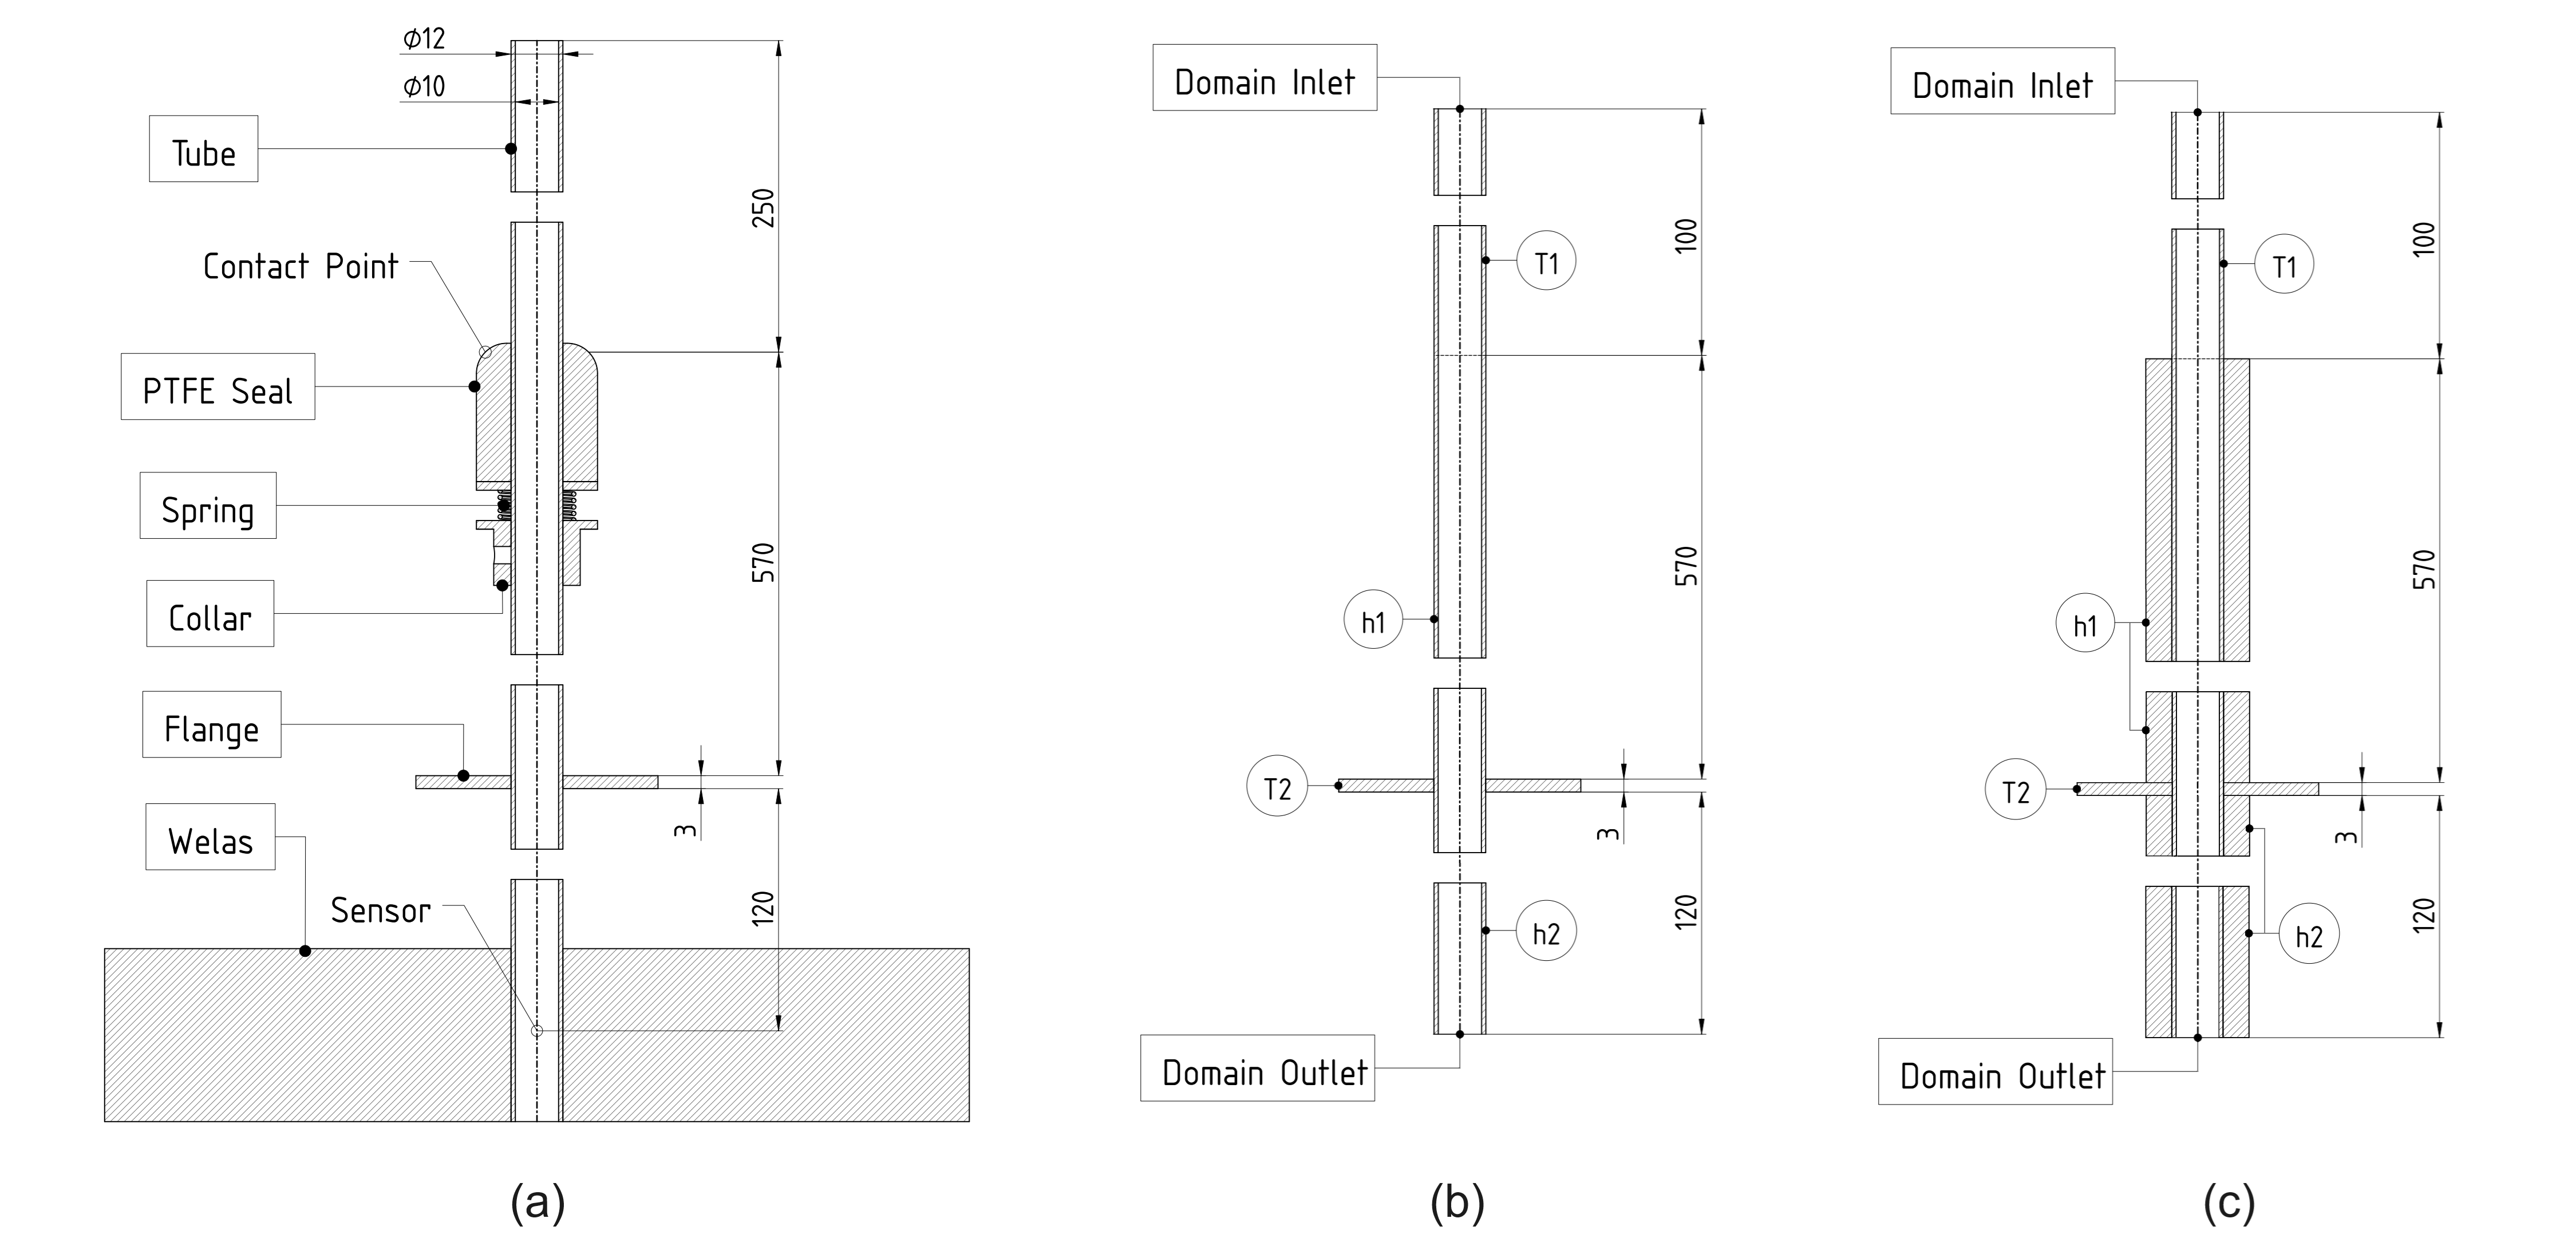
\includegraphics[width=1\linewidth]{figures/geometries-1.2.png}
        \caption{Geometry analyzed: (a) real geometry, (b) simplified geometry without isolation, and (c) simplified geometry with isolation. Dimensions, components, and boundary conditions are indicated.}
        \label{fig:figure1}
    \end{figure}

\end{frame}


\subsection{Ecuaciones}
\begin{frame}{Fórmulas Matemáticas}

Ejemplos :

\begin{itemize}
    \item Ecuación de la energía: 
    \[
    \frac{dE}{dt} = P - \dot{Q}
    \]
    donde \( P \) es la potencia y \( \dot{Q} \) es la tasa de transferencia de calor.

    \item Ecuación de la ecuación de calor unidimensional:
    \[
    \frac{\partial T}{\partial t} = \alpha \frac{\partial^2 T}{\partial x^2}
    \]
    donde \( \alpha \) es la difusividad térmica.

    \item La ecuación de la conservación de la masa:
    \[
    \nabla \cdot \vec{v} = 0
    \]
\end{itemize}

\end{frame}


\begin{frame}[fragile]
\frametitle{Código en Python}
\scriptsize
% \tiny % tamano de letra más chico, para toda la slide

A continuación, se muestra un ejemplo de código en Python:

    \begin{lstlisting}[language=Python, style=pythonstyle]
    # Este es un ejemplo de Python
    def suma(a, b):
        return a + b
    
    resultado = suma(5, 3)
    print("El resultado es:", resultado)
    \end{lstlisting}

\end{frame}

\end{document}
